\documentclass{article}

\usepackage{lmodern}
\usepackage{hyperref}
\usepackage{amsmath}
\usepackage{amssymb}
\usepackage[T1]{fontenc}
\usepackage{fancyhdr}
\usepackage{color,graphicx}
\pagestyle{fancy}
\lhead{Anirudhan J. Rajagopalan --- ajr619}
\lhead{Michele Ceru --- mc3784}

\begin{document}

\title{Deep Learning --- Homework 1}
\date{February 11, 2016}
\author{Anirudhan J. Rajagopalan, Michele Ceru\\ ajr619, mc3784}

\maketitle

\newpage

\section[Expression for energy]{Backpropogation}
\begin{enumerate}
\item Using the chain rule:
$$
\frac{\partial E}{\partial x_{\text{in}}} = \frac{\partial E}{\partial x_{\text{out}}}\frac{\partial x_{\text{out}}}{\partial x_{\text{in}}}
$$  
Using the expression of $x_{\text{out}}$ given in the question we have:
$$
\frac{\partial x_{\text{out}}}{\partial x_{\text{in}}} = \frac{\partial }{\partial x_{\text{in}}} \big(\frac{1}{1+e^{-x_{\text{in}}}}\big) = \frac{e^{-x_{\text{in}}} }{(1+e^{-x_{\text{in}}})^2}
$$
Summing and subtracting $1$ in the numerator:
$$
\frac{\partial x_{\text{out}}}{\partial x_{\text{in}}}  = \frac{1+e^{-x_{\text{in}}} -1}{(1+e^{-x_{\text{in}}})^2}=\frac{1}{1-e^{-x_{\text{in}}}}\Big[  1-\frac{1}{1-e^{-x_{\text{in}}}}\Big]
$$
And using the expression of $x_{\text{out}}$ given in the question:
$$
\frac{\partial E}{\partial x_{\text{in}}} =\frac{\partial E}{\partial x_{\text{out}}}x_{\text{out}}[1-x_{\text{out}}]
$$

\item Using the expression of $x_{\text{out}}$ given in the question:
$$
\frac{\partial (x_{\text{out}})_i}{\partial (x_{\text{in}})_j} = \frac{\partial }{\partial (x_{\text{in}})_j} \Big(  
\frac{e^{-\beta (x_{\text{in}})_i}}{\sum_k e^{-\beta (x_{\text{in}})_k}}
\Big)
$$
In the case $i=j$:
$$
\frac{\partial (x_{\text{out}})_i}{\partial (x_{\text{in}})_i} =    
\frac{-\beta e^{-\beta (x_{\text{in}})_i} (\sum_k e^{-\beta (x_{\text{in}})_k} )- e^{-\beta (x_{\text{in}})_i} (-\beta e^{-\beta (x_{\text{in}})_i}   )
}
{\sum_k e^{-\beta (x_{\text{in}})_k}}=
$$

$$
=-\frac{\beta e^{-\beta (x_{\text{in}})_i}}{\sum_k e^{-\beta (x_{\text{in}})_k} } \Big[  1-\frac{\beta e^{-\beta (x_{\text{in}})_i}}{\sum_k e^{-\beta (x_{\text{in}})_k} }\Big]
$$and substituting the expression of $x_{\text{out}}$:
$$
\frac{\partial (x_{\text{out}})_i}{\partial (x_{\text{in}})_i} =\beta  (x_{\text{out}})_i [1- (x_{\text{out}})_i]
$$
In the case $i\neq j$:
$$
\frac{\partial (x_{\text{out}})_i}{\partial (x_{\text{in}})_j} =    
-\beta e^{-\beta (x_{\text{in}})_j} (\sum_k e^{-\beta (x_{\text{in}})_k} )^{-2} e^{-\beta (x_{\text{in}})_i} =
$$ 
$$
=\beta \frac{e^{-\beta (x_{\text{in}})_j}}{\sum_k e^{-\beta (x_{\text{in}})_k} }
\frac{e^{-\beta (x_{\text{in}})_i}}{\sum_k e^{-\beta (x_{\text{in}})_k} } =\beta (x_{\text{out}})_j(x_{\text{out}})_i 
$$
Writing the solution all together:
\begin{equation*}
      \frac{\partial (x_{\text{out}})_i}{\partial (x_{\text{in}})_j} = \begin{cases}
                       \beta  (x_{\text{out}})_i [1- (x_{\text{out}})_i]   \text{\,	if  $i= j$}\\
                        \beta (x_{\text{out}})_j(x_{\text{out}})_i   \text{\,	if  $i\neq j$}
                    \end{cases}
\end{equation*}

\end{enumerate}

\section[Kaggle contest]{Torch (MNIST handwriting recognition)}

\subsubsection{Model file}
  The model file can be found at \href{http://cs.nyu.edu/\textasciitilde ajr619/model.net}{http://cs.nyu.edu/\textasciitilde ajr619/model.net}
\subsubsection{Github repo}
  The repository for the changes and result.lua is at \\
  \href{https://github.com/rajegannathan/Deep-Learning/tree/master/hw1}{https://github.com/rajegannathan/Deep-Learning/tree/master/hw1}
\subsubsection{Best performing model}
We got a best test set performance of 99.63\%.  We added Gaussian noise to all the images, followed by randomly rotating the image by an angle derived from a gaussian distribution of mean 0 and deviation 0.174 (corresponding to 10 degree rotation).  We also added a convolutional layer along with dropout.  Though we achieved best performance with this layer, we got almost similar performance of 99.62\% with just the image rotation.
\subsubsection{Experiments}
  We ran a number of experiments starting with tweakign the options being passed to the test, train and model lua scripts.
\begin{description}

  \item[SGD Batch size:] Changing the batch size of SGD decreases the performance drastically.  For batch size of 32, 64 and 128 the model's accuracy was in the range of 78\%, 60\% and  45\% respectively.

  \item[Momentum and Learning rate:] Theoretically, using a value of momentum greater than zero (and lesser than one) should help us jump over local minimum.  When combined with proper value of learning rate we should be able to find a non local minimum.  But from our experiments, we were unable to find a good combination of learning rate and momentum that gives a better performance than the default momentum of zero and learning rate of $10^{-3} $.  The performance drop was considerable and we were able to achieve accuracy in the range of around ~30\% only.

  \item[Optimization algorithm] Another theoritical point which we considered was to use SGD in the starting few epoches and then switch the optimization algorithm to something better such as BFGS.  Theoretically, SGD is supposed to help us skip saddle points and once we are near a minima, the other optimization algorithm could help us converge faster.  So we tried experimenting by changing the optimization algorithm after epochs 5, 7, 15 and 30.  We were able to get performance on par with the default SGD implementation (99.2\% accuracy) and we didn't observe any improvements in performance.
  
\item[Data Augmentation]  To generate more training examples we rotated the training data of random angle. The chosen criteria to rotate the image is a normal distribution with zero mean and $\theta$ standard deviation. During the training we rotated al the images randomly using this normal distribution. We run experiment with different values of $\theta$, noticing that the performance improve for values smaller than  $20$ degree. In particular we found our best performance for $\theta=0.174$, that is around $11.46$ degree.

\item[Introduction of noise] In order to reduce overfitting we introduced a random gaussian noise in the training images. Doing so, we obtained an overall worse performance during the training phase and a comparable performance during the testing phase, reducing in such way the gap of the performance between training and testing .

\item[Additional Convolutional layer] We added an additional spatial convolutional layer, but we didn't notice any considerable improvement.

\item[Drop out] Added a drop out layer along with the additional convolutional layer.

\item[Other experiments]
    We also tried with other optimization routines such as ASGD and CG.  But the script was giving a number of exceptions and we didn't explore it further due to time constraints.

\end{description}
\subsubsection{Figures}
\begin{figure}[ht!]
  \centering
  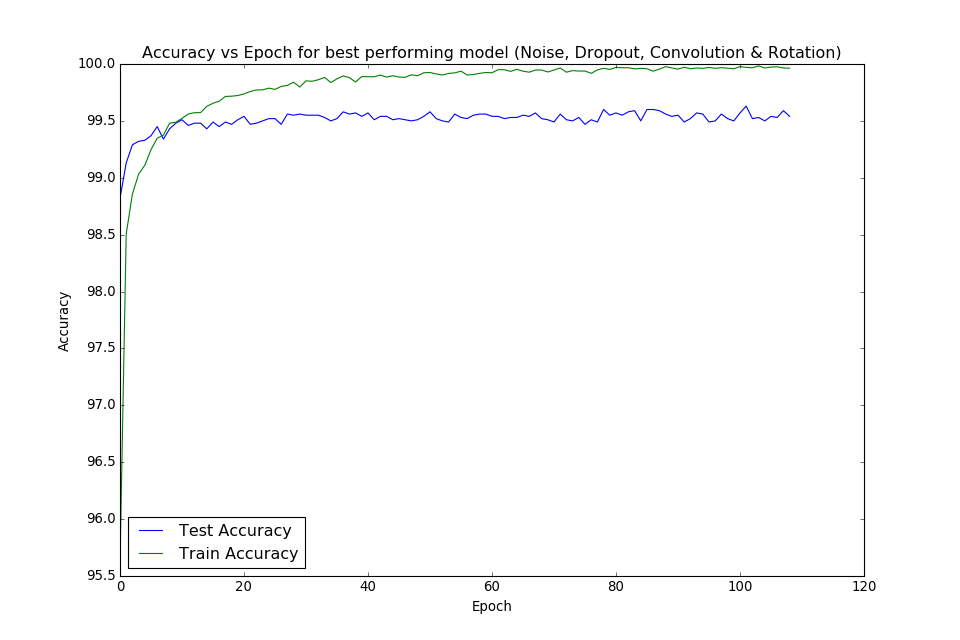
\includegraphics[width=0.65\textwidth]{topperformance}
  \caption{Best performance figures. We used a network architecture that adds noise to the image, rotates the images by random angles drawn from a normal distribution with zero mean and 0.174 standard deviation and also has a convolution and dropout layers..\label{fig:top_performance}}
\end{figure}
\begin{figure}[ht!]
  \centering
  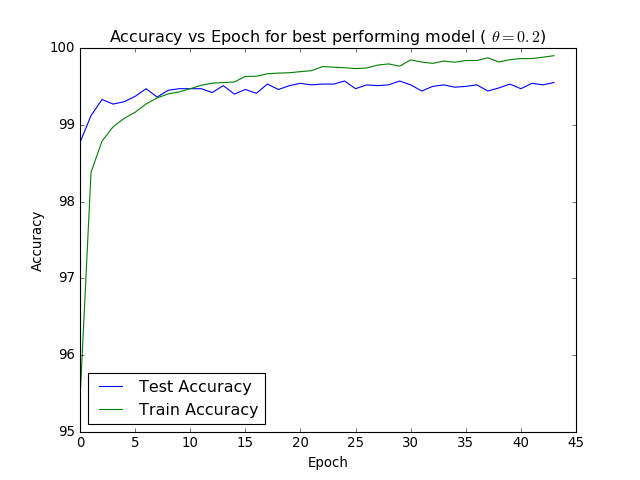
\includegraphics[width=0.65\textwidth]{bestPerformance}
  \caption{Second best performance figures. We added a layer that rotates the images by random angles drawn from a normal distribution with zero mean and 0.2 standard deviation. \label{fig:best_performance}}
\end{figure}
\begin{figure}[ht!]
  \centering
  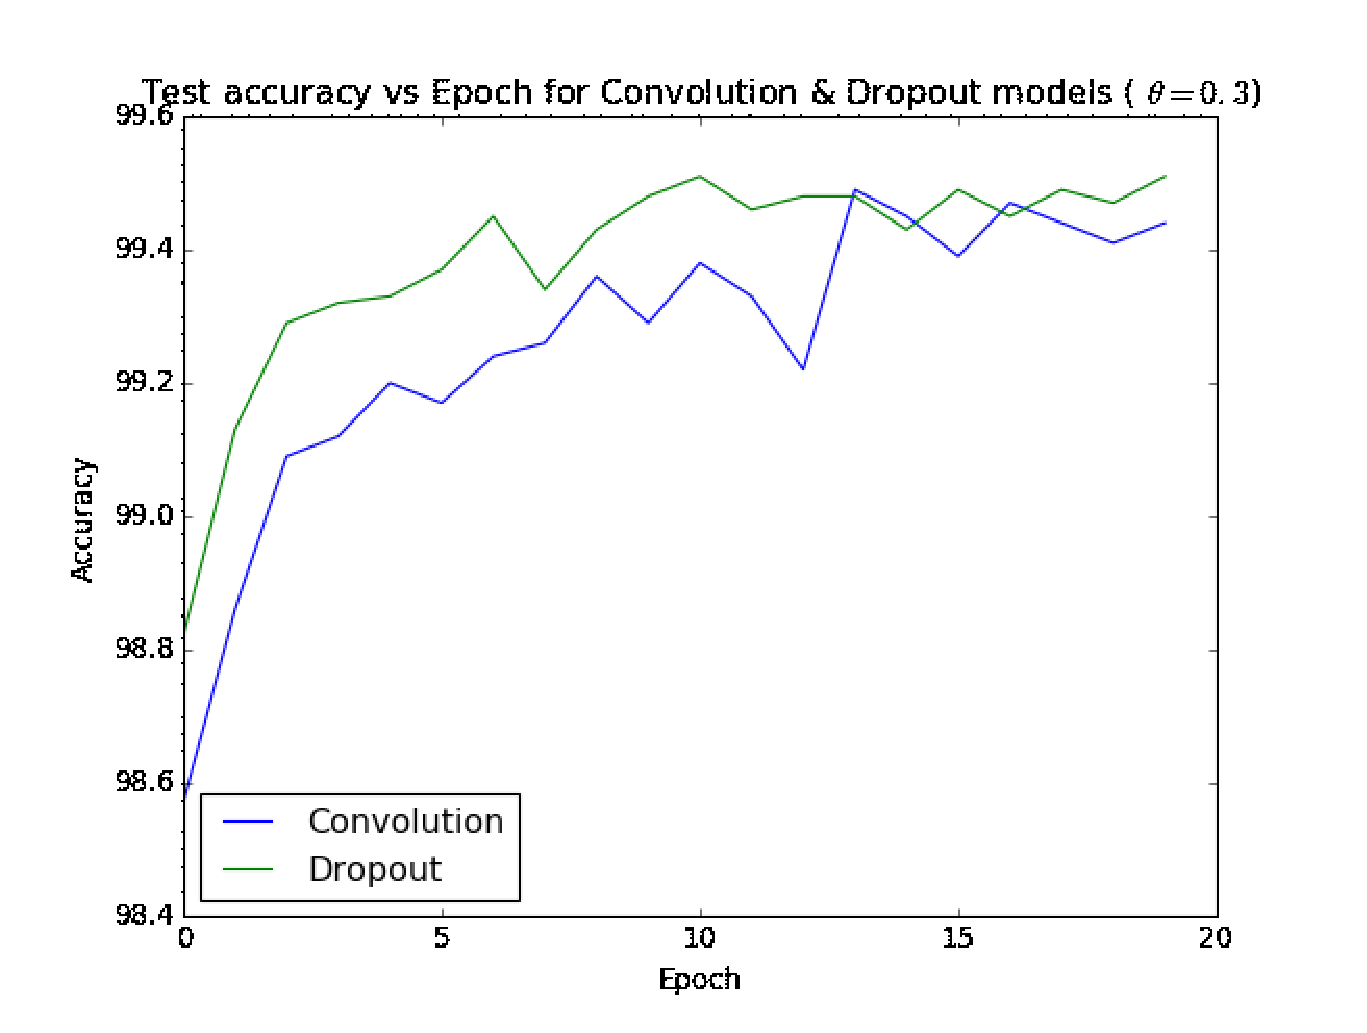
\includegraphics[width=0.65\textwidth]{convolution_dropout}
  \caption{Adding convolutional layers and dropout model to the model with 0.2 rotation. \label{fig:convolution_dropout}}
\end{figure}
\end{document}
